---
title: 初等部分構造を用いたErdős-Radoの定理の証明
author: 石井 大海
tag: 数学,数理論理学,集合論,モデル理論,無限組合せ論,Erdős-Radoの定理,Ramsey理論,Ramseyの定理,ゼミ資料,ラムゼーの定理,ラムゼー理論,エルデシュ・ラドーの定理,エルデシュ,ラドー,ラムゼー,エルデシュ=ラドーの定理
latexmk: -pdflua
description: Erdős-Radoの定理はRamseyの定理に代表されるような,無限組合せ論における分割・彩色性質の一つです.ここではオリジナルの純粋に組合せ論的な証明ではなく,初等部分構造を用いたより簡単な方法を紹介します.
date: 2014/05/01 23:00:42 JST
---
\documentclass[a4j,lualatex,ja=standard]{bxjsarticle}
\usepackage[hiragino-pron]{luatexja-preset}
\usepackage{tikz}
\usetikzlibrary{arrows}
\usepackage{amsmath,amssymb}
\usepackage{mystyle}
\usepackage[pdfauthor={石井大海},%
            pdftitle={初等部分構造を用いたErdős-Radoの定理の証明}]{hyperref}
\usepackage[backend=biber, style=numeric]{biblatex}
\addbibresource{myreference.bib}
\newcommand{\Erdos}{Erd\H{o}s}
\title{初等部分構造を用いた\Erdos-Radoの定理の証明}
\author{石井大海}
\date{2014/05/01 23:00:42 JST}

\begin{document}
\maketitle

※これは研究室でのゼミ資料を一部改変して公開したものである.
\section{定義と準備}
以下では,初等部分構造を用いた議論をするので,まずその準備をしておく:
\begin{definition}
 $\kappa \geq \omega$とする.$M$が$\kappa$-{\itshape closed} $\Leftrightarrow [M]^{<\kappa} \subseteq M$
\end{definition}

\begin{lemma}\label{lem:LS-generalized}
 $\theta > \kappa \geq \omega$とする.$S \in [H(\theta)]^{\leq 2^\kappa}$とおくと,$M \preccurlyeq H(\theta)$で次を満たすものが存在する:
 \begin{enumerate}
  \item $S \subseteq M$
  \item $M$は$\kappa^+$-closed
  \item $|M| = 2^\kappa$
 \end{enumerate}
\end{lemma}
\begin{proof}
 L\"{o}wenheim-Skolemの定理より$M_0 \preccurlyeq H(\theta)$で$S \subseteq M_0$かつ$|M_0| = |S| = 2^\kappa$を満たすものが取れる.$M_\alpha \preccurlyeq M_\beta \preccurlyeq H(\theta), |M_\alpha| = 2^\kappa\; (\alpha < \beta < \kappa^+)$なる初等鎖を構成できれば,$M = \bigcup_{\alpha < \kappa^+} M_\alpha$が求める物となる.まず,$\alpha$が極限順序数の時には$M_\alpha = \bigcup_{\beta < \alpha} M_\beta$と置けば,初等鎖定理より$\beta < \alpha \rightarrow M_\beta \preccurlyeq M_\alpha$となり,濃度の条件もOK.つづいて$\alpha = \beta + 1$ とする.この時,$(2^{\kappa})^{<\kappa^+} =(2^\kappa)^{\leq \kappa} = 2^{\kappa \kappa} = 2^\kappa$に注意すれば,$S_\alpha = M_\beta \cup [M_\beta]^{<\kappa^+}$の濃度は$2^\kappa$である.そこでL\"{o}wenheim-Skolemの定理により$S_\alpha \subseteq M_\alpha \preccurlyeq H(\theta), |M_\alpha| = 2^\kappa$なる$M_\alpha$を取れば良い.\mbox{}
\end{proof}
\begin{definition}
 $\kappa \geq \lambda, \sigma$を基数,$n<\omega$とする.この時,
 \[
 \kappa \longrightarrow (\lambda)^n_\sigma
 \defs \forall f: [\kappa]^n \to \sigma\, \exists Z \in [\kappa]^\lambda\, \forall A, B \in [Z]^n \left[ f(A) = f(B)\right]
 \]
 各$f$に対する$Z$を,分割$f$に関する{\bfseries 等質集合}({\itshape homogeneous set})と呼ぶ.
\end{definition}

\begin{rem*}
 \begin{itemize}
  \item $\kappa' \geq \kappa, \lambda' \leq \lambda, \sigma' \leq \sigma, \kappa \longrightarrow (\lambda)^n_\sigma
	\Longrightarrow \kappa' \longrightarrow (\lambda')^n_{\sigma'}$
  \item ここでは無限組合せ論的性質を見たいので,$\kappa, \lambda \geq \omega$の場合だけを考える
  \item $\lambda > \kappa$の時は$[\kappa]^\lambda = \emptyset$となり自明.
  \item $\sigma \geq \kappa$の時は,$[\kappa]^n \congto \kappa \xrightarrow[]{id} \sigma$を考えれば明らかに偽.よって以下$\sigma < \kappa$とする.
  \item $n = 0$の時は自明
 \end{itemize}
\end{rem*}

\begin{lemma}\label{er:small}
 $\kappa \geq \lambda \geq \omega$の時,次が成立:
 \[
  \kappa \longrightarrow (\lambda)^1_\sigma
 \Leftrightarrow \begin{cases}
		  \sigma < \cf(\kappa) & (\kappa = \lambda)\\
		  \sigma < \kappa      & (\kappa > \lambda)
		 \end{cases}
 \]
\end{lemma}
\begin{proof}
 $n = 1$のとき,$\kappa \longrightarrow (\lambda)^1_\sigma$は次と同値であることが判る:
 \[
  \forall f : \kappa \rightarrow \sigma \, \exists \alpha < \sigma \, (|f^{-1}[\{\alpha\}]| \geq \lambda)
 \]
 
 まずは$\kappa = \lambda$の時を考え,対偶を示す.
 $\sigma \geq \cf(\kappa)$の時,$A = \Set{a_\alpha : \alpha < \sigma} \in [\kappa]^\sigma$を$\kappa$の共終部分集合とする.$f : \kappa \rightarrow \sigma$を$f(\alpha) = \min \Set{\gamma | \alpha \leq a_\gamma}$により定める.すると,各$\gamma < \sigma$に対し$|f^{-1}[\{\gamma\}]| \leq |a_\gamma| < \kappa$となるので$\kappa \nrightarrow (\kappa)^1_\sigma$.逆に$\kappa \nrightarrow (\kappa)^1_\sigma$とする.$f: \kappa \rightarrow \sigma$を$|f^{-1}[\{\beta\}]| < \kappa$を満たすようなものとする.この時$\kappa = \bigcup_{\beta < \sigma} f^{-1}[\{\beta\}]$より$\sigma \geq \cf(\sigma)$となる.よって示された.

 今度は$\lambda < \kappa$とし対偶を示す.$\sigma = \kappa$とすると,恒等関数$id: \kappa \rightarrow \kappa$を考えれば$f^{-1}[\{\alpha\}] = \{\alpha\}$より$\kappa \nrightarrow (\lambda)^1_\kappa$である.逆に,$\kappa \nrightarrow (\lambda)^1_\sigma$とし,$f : \kappa \rightarrow \sigma$が$|f^{-1}[\{\alpha\}]| < \lambda$を満たすとする.
 \[
  \kappa = \left|\bigcup_{\beta < \sigma} f^{-1}[\{\beta\}]\right| = \max\left\{ \sigma, \sup_{\beta < \sigma} \left|f^{-1}[\{\beta\}]\right| \right\}
 \]
 ここで$|f^{-1}[\{a\}]| < \lambda$より$\sup_{\alpha < \sigma} |f^{-1}[\{\alpha\}]| \leq \lambda < \kappa$となる事に注意すれば,$\kappa = \sigma$となる.\mbox{}
\end{proof}

よって,$n = 0, 1$の時の$\kappa \longrightarrow (\lambda)^n_\sigma$はかなり簡単になるので,興味があるのは$n \geq 2$の時である.次はRamseyによる古典的な結果である.本筋の命題ではないので,証明は概略に留める:
\begin{theorem}[Ramsey]
 $\forall n, k < \omega\, [\omega \longrightarrow (\omega)^n_k]$
\end{theorem}
\begin{proof}[証明の概略]
 $n$に関する帰納法で示す.$n = 0$は先程の議論より自明.$n$の時成立を仮定し,$n+1$の場合を考える.$f: [\omega]^{n+1} \rightarrow k$を固定し,各$x \in \omega$に対し,$f_x : [\omega \setminus \{x\}]^n \rightarrow k$を$f_x(A) = f(A \cup \set{x})$により定める.次を満たす$H_\ell \in [\omega]^\omega, x_\ell < \omega, i_\ell < k$を帰納的に構成する:
 \begin{enumerate}[label=(\alph*)]
  \item $H_\ell \supseteq H_{\ell+1}$
  \item $\Set{x_\ell : \ell \leq n} \cap H_{n} = \emptyset$
  \item $x_\ell \in H_{\ell - 1}\, (\ell \geq 1)$
  \item $f_{x_\ell}\left[[H_\ell]^n\right] = \{i_\ell\}$
 \end{enumerate}
 すると,$L = \Set{\ell < \omega : i_\ell = i}$が無限集合になるような$i < k$が少なくとも一つ存在する.この時,$H = \Set{x_\ell : \ell \in L}$が求めるものとなる.\mbox{}
\end{proof}

よって特に$\omega \longrightarrow (\omega)^2_2$.では,等質集合の濃度が非可算となるような,即ち$\kappa \longrightarrow (\omega_1)^2_2$が成り立つような$\kappa$はどんなものがあるだろうか?実は$(2^\omega)^+$で十分である:

\begin{theorem}
 $(2^\omega)^+ \longrightarrow (\omega_1)^2_\omega$.よって特に$(2^\omega)^+ \longrightarrow (\omega_1)^2_2$.
\end{theorem}

これは次のErd\H{o}s-Radoの定理で$n=1, \kappa = \omega$とおけば直ちに従う:

\begin{theorem}[一般化\Erdos-Rado]\label{Th:E-R}
 $\kappa \geq \omega$とする.
 \[
  \mathrm{exp}_0(\kappa) = \kappa, \mathrm{exp}_{n+1}(\kappa) = 2^{\exp_n(\kappa)}
 \]
 と表すとき,次が成立:
 \[
  (\mathrm{exp}_{n}(\kappa))^+ \longrightarrow (\kappa^+)^{n+1}_\kappa
 \]
\end{theorem}

\begin{proof}
 $n$に関する帰納法で証明する.$n = 0$の時は$\kappa^+ \longrightarrow (\kappa^+)^1_\kappa$であり,$\kappa < \kappa^+ = \cf(\kappa^+)$なので補題 \ref{er:small}より成立.

$n+1$の場合を考える.以後,簡単の為$\mathrm{exp}_n(\kappa) = \chi_n$と略記する.帰納法の仮定は,
\[
 (\chi_n)^+ \longrightarrow (\kappa^+)^{n+1}_\kappa
\]
である.$f: [\chi_{n+1}^+]^{n+2} \longrightarrow \kappa$を固定し,$Z \in [\chi_{n+1}^+]^{\kappa^+}$で$f$について等質となるものを得たい.そこで,まず$f, \chi_{n+1}^+ \in H(\theta), \kappa \subseteq H(\theta)$を満たす十分大きな$\theta > \omega$を取り,その$\chi_n^+$-closedな初等部分構造$M \preccurlyeq H(\theta)$で$f, \chi_{n+1}^+ \in M$かつ$\kappa \subseteq M$となるものを取る.補題 \ref{lem:LS-generalized} より,特に$|M| = 2^{\chi_n} = \chi_{n+1}$とできる.すると,$|M \cap \chi_{n+1}^+| \leq \chi_{n+1}$となり,$\chi_{n+1}^+$の正則性より$j = \sup^+(\chi_{n+1}^+ \cap M) \in \chi_{n+1}^+$が取れる.

 以下,各$\xi < \chi_{n}^+$に対し,
 \[
 \forall \eta < \xi \, [ i_\eta < i_\xi] \wedge \forall \eta_0, \dots, \eta_n < \xi \, [f(\{i_{\eta_0}, \dots, i_{\eta_n}, i_\xi\}) = f(\{i_{\eta_0}, \dots, i_{\eta_n}, j\})]
 \]
 を満たすよう帰納的に$\Braket{i_\xi \in \chi_{n+1}^+ \cap M | \xi < \chi_n^+}$を定めたい.そこで,$\xi$未満まで出来たとし,$D = \Set{ i_\eta : \eta < \xi} \subseteq M \cap \chi_{n+1}^+$とおく.この時$|D| = |\xi| < \chi_n^+$なので,$M$の$\chi_n^+$-closed性から$D \in M$となる.また,$M$は有限部分集合について閉じるから,$D \subseteq M$より$[D]^{n+1} \subseteq M$となり,更に$|[D]^{n+1}| = |D| < \chi_n^+$から$[D]^{n+1} \in M$も云える.そこで,$g : [D]^{n+1} \rightarrow \kappa$を$g(A) = f(A \cup \{j\})$により定める.すると,$\kappa \subseteq M$となるように取っており,$H(\theta)$で$\mathrm{ZFC}-\mathrm{P}$(特に対の公理)が成り立つことから$[D]^{n+1} \times \kappa \subseteq M$.よって$g \subseteq [D]^{n+1} \times \kappa \subseteq M$となり,特に$|g| < \chi_n^+$だからみたび$M$の$\chi_n^+$-closed性より$g \in M$が言える.今,
 \[
  H(\theta) \models
 \exists y \in \chi_{n+1}^+\;\left[ \forall i \in D\, (i < y) \wedge \forall A \in [D]^{n+1}\, (f(A \cup \{y\}) = g(A))\right]
 \]
 が成立する($y$として$j$が取れる).この右辺の論理式に現れるパラメータ$\chi_{n+1}^+, D, [D]^{n+1}, f, g$は全て$M$の元であり,$M \preccurlyeq H(\theta)$であるので,$M$でも成立する.そこで$i_\xi$としてそのような$y$を取れば良い.

 $W = \Set{ i_\xi : \xi < \chi_n^+}$と置く.この時$f_j(A) = f(A \cup \{j\})$により$f_j: [W]^{n+1} \rightarrow \kappa$を定める.帰納法の仮定を分割$f_j$と$W$に適用すれば,$Z \in [W]^{\kappa^+}, \alpha < \kappa$で$f_j[[Z]^{n+1}] = \{\alpha\}$となるような物が取れる.この時,$A = \{i_{\xi_0} < \dots < i_{\xi_n} < i_{\xi_{n+1}}\} \in [Z]^{n+2}\;(\xi_k < \xi_{k+1})$を任意に取れば,
 \[
  f(A) = f(\{i_{\xi_0}, \dots, i_{\xi_n}, i_{\xi_{n+1}}\})
 = f(\{i_{\xi_0}, \dots, i_{\xi_n}, j\})
 = f_j(\{i_{\xi_0}, \dots, i_{\xi_n}\}) = \alpha
 \]
 ここで$A = \set{i_{\xi_0}, \dots, i_{\xi_{n+1}}}$の取り方は任意なので,$Z$は$f$について等質であることが示せた.\mbox{}
\end{proof}

\section{関連する問題}
\subsection{$(2^\omega)^+$が最小であること}
上での議論から,$\kappa \geq (2^\omega)^+$ならば$\kappa \longrightarrow (\omega_1)^2_2$が成立することがわかる.この値は最小なのだろうか?次のSierpinskiの議論から,$2^\omega$では不十分であり,この結果がoptimalであることがわかる:
\begin{lemma}[Sierpinski]
 $2^\omega \nrightarrow (\omega_1)^2_2$
\end{lemma}
より一般に,次が成り立つ:
\begin{lemma}[Sierpinski]
 $\kappa \geq \omega$に対し,$2^\kappa \nrightarrow (\kappa^+)^2_2$.よって特に$2^\kappa \nrightarrow (\kappa^+)^2_\kappa$.
\end{lemma}
\begin{proof}
 問題になるのは濃度だけなので,$\power{\kappa}{2}$を考える.$<$を$\power{\kappa}{2}$上の辞書式順序,$\lhd$を$\power{\kappa}{2}$上のある整列順序とする.この時,関数$f : [\power{\kappa}{2}]^2 \rightarrow 2$を次で定義する:
 \[
  f(\{x, y\}) \defeq \begin{cases}
		      0 & (x < y \Leftrightarrow x \lhd y)\\
		      1 & (otherwise)
		     \end{cases}
 \]
 もし分割$f$に関する等質集合$Z \in [\power{\kappa}{2}]^{\kappa^+}$が存在したとすれば,$Z$は辞書式順序$<$またはその逆順序$>$により整列され,特に$\kappa^+$-型の昇鎖または降鎖を含むことになる.次の主張を示せば証明は完了する:

\begin{claim}
 $\kappa \geq \omega$とする.$\power{\kappa}{2}$は辞書式順序$<$に関する$\kappa^+$-型の降鎖・昇鎖を持たない.
\end{claim}
昇鎖でも降鎖でも議論は同じなので,以下昇鎖の場合を考える.$\Braket{f_\alpha | \alpha < \kappa^+}$を$f_\alpha < f_\beta \; (\alpha < \beta)$を満たす$\power{\kappa}{2}$の昇鎖とする.この時,$\gamma \leq \kappa$を$\Set{ f_\alpha \restr \gamma : \alpha < \kappa^+}$が濃度$\kappa^+$となるような最小の物とする.そこで,最初の昇鎖は$f_\alpha \restr \gamma = f_\beta \restr \gamma \Rightarrow f_\alpha = f_\beta$を満たすとして一般性を失わない.

各$\alpha < \kappa^+$に対し,$f_\alpha \restr \xi_\alpha = f_{\alpha+1} \restr \xi_\alpha$かつ$f_\alpha(\xi_\alpha) = 0, f_{\alpha+1}(\xi_\alpha) = 1$となるような$\xi_\alpha$を取る.これは辞書式順序の定義から一意に定まる.$\gamma \leq \xi_\alpha$とすると$f_\alpha \restr \xi_\alpha \neq f_{\alpha+1} \restr \xi_\alpha$となってしまうので,$\xi_\alpha < \gamma$であることに注意しよう.この時,$\kappa^+$の正則性より$A = \Set{\alpha < \kappa^+ : \xi_\alpha = \xi}$の濃度が$\kappa^+$になるような$\xi < \gamma < \kappa^+$が取れる.$\alpha, \beta \in A$かつ$f_\alpha \restr \xi = f_\beta \restr \xi$とする.このとき$\xi = \xi_\alpha = \xi_\beta$なので,$f_{\alpha+1} \restr \xi_\beta = f_{\alpha+1} \restr \xi_\alpha = f_\alpha \restr \xi_\alpha = f_\beta \restr \xi_\beta$となる.また$\xi_\alpha$の取り方より$f_{\alpha+1}(\xi_{\beta}) = 1$である.このような条件を満たす$\delta$の中で$\beta+1$は最小なので,$\beta+1 \leq \alpha+1$となる.同様の議論により$\alpha+1\leq\beta+1$となり,従って$\alpha=\beta$となる.よって,$\Set{f_\alpha \restr \xi : \alpha \in A}$の濃度は$\kappa^+$である.しかし,これは$\gamma$の最小性に反する.\mbox{}
\end{proof}

\subsection{有限組合せ論}
$\kappa, \lambda < \omega$ の場合は(有限)組合せ論の非自明な問題である.以下に二つだけ例を挙げる:
 \begin{itemize}
   \item $6 \longrightarrow (3)^2_2$は成立する
	 \begin{center}
	  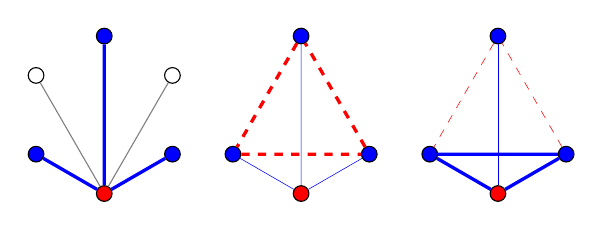
\begin{tikzpicture}
	   \begin{scope}
 	   \node (p0) at (270:1cm) 
	     [inner sep=2pt,circle,draw=black,fill=red] {};
	   \foreach \x in {1,...,5} {
	     \pgfmathparse{mod(\x,2) ? "blue" : "white"}
	     \edef\col{\pgfmathresult}
	     \node (p\x) at ({270+60*\x}:1cm)
	      [inner sep=2pt,circle,draw=black,fill=\col] {};
	   }
	   \draw [blue, very thick]
	     (p0) -- (p1)
	     (p0) -- (p3)
	     (p0) -- (p5);
	   \draw [gray,thin]
	     (p0) -- (p2)
	     (p0) -- (p4);
	   \end{scope}	  
	   \begin{scope}[xshift=2.5cm]
 	   \node (p0) at (270:1cm) 
	     [inner sep=2pt,circle,draw=black,fill=red] {};
	   \foreach \x in {1,3,5} {
	     \node (p\x) at ({330+240*\x}:1cm)
	      [inner sep=2pt,circle,draw=black,fill=blue] {};
	   }
	   \draw [blue,very thin]
	     (p0) -- (p1)
	     (p0) -- (p3)
	     (p0) -- (p5);
	   \draw [dashed ,very thick,red]
	     (p5) -- (p1)
	     (p1) -- (p3)
	     (p3) -- (p5);
	   \end{scope}	  
	  \begin{scope}[xshift=5cm]
 	   \node (p0) at (270:1cm) 
	     [inner sep=2pt,circle,draw=black,fill=red] {};
	   \foreach \x in {1,3,5} {
	     \node (p\x) at ({330+240*\x}:1cm)
	      [inner sep=2pt,circle,draw=black,fill=blue] {};
	   }
	   \draw [blue, very thick]
	     (p0) -- (p1)
	     (p0) -- (p3)
	     (p1) -- (p3);
	   \draw [blue,very thin]
	     (p0) -- (p5);
	   \draw [dashed,very thin,red]
	     (p5) -- (p1)
	     (p3) -- (p5);	  
	  \end{scope}	  
	  \end{tikzpicture}
	 \end{center}

   \item $5 \nrightarrow (3)^2_2$:次の図が反例(どの三角形も異なる色の辺を含む):
	 \begin{center}
	  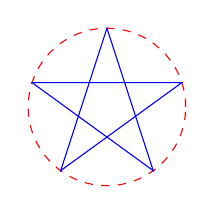
\begin{tikzpicture}
	   \draw[dashed, red] (0,0) circle (1cm);
	   \draw[blue] (18:1cm) \foreach \x in {162,306,...,738} {
	    -- (\x:1cm)
	   } -- cycle;
	  \end{tikzpicture}
	 \end{center}
 \end{itemize}

\nocite{Kunen:2011,Jech:2002,Kanamori:2009,Negami:1990,Tanaka:2011}
\printbibliography[title=参考文献]
\end{document}
